\documentclass{article}
\usepackage[preprint]{neurips_2024}

\usepackage[utf8]{inputenc}
\usepackage[T1]{fontenc}
\usepackage{graphicx}
\usepackage{booktabs}
\usepackage{amsfonts}
\usepackage{amsmath}
\usepackage{tikz}
\usetikzlibrary{arrows.meta, positioning, fit}

\title{Provenance-Chained Résumé Optimization:\\
A System for Verified ATS-Calibrated Rewriting}

\author{
  [Author Name] \\
  [Affiliation] \\
  \texttt{[email@domain]}
}

\begin{document}

\maketitle

\begin{abstract}
Large language models make résumé parsing and rewriting easy to prototype and dangerous to ship:
a rewriter that fabricates an employer, a skill, or a metric produces a résumé that reads better
and lies. We present a résumé-optimization system built around three properties that we argue are
necessary, not optional, for this task. \textbf{(C1) A continuous provenance chain}: every field
extracted from a résumé carries a stable identifier pointing to its exact source span, and that
identifier survives unbroken through matching, scoring, and rewriting. \textbf{(C2) Real-engine
ATS-calibrated scoring}: rather than reporting a cosine-similarity proxy, we calibrate a
$0$--$100$ match score against the actual parse-and-match output of a self-hostable, rule-based
ATS simulator. \textbf{(C3) A provenance-verified rewrite gate}: every edit the rewriter proposes
must resolve to a source provenance identifier or is rejected before it reaches the output, with a
fabrication rate reported rather than assumed away. The system is orchestrated as a
seven-node graph with two parallel branches (résumé parsing, job-description analysis) that fan in
at a matching stage, followed by calibrated scoring, gated rewriting, and a reviewer node that
independently re-asserts the provenance invariant on the shipped output. We report results with
\texttt{gemini-3.1-flash-lite} as the primary inference backend across three tasks --
extraction quality (288/300 documents from three gold sets), ATS-score calibration (199 real
résumé--job-description pairs), and the fabrication gate (30 adversarial pairs) -- and confirm
that the central guarantee, zero unsourced additions reaching a shipped rewrite, holds identically
when the same pipeline is run on a locally-hosted \texttt{qwen2.5:14b}. We also report and analyze
a genuine, reproducible failure mode of the primary backend: a deterministic generation loop that
truncates extraction output on a specific class of ambiguously-formatted résumé dates.
\end{abstract}

\section{Introduction}

Résumé optimization -- taking a candidate's résumé and a target job description and producing a
tailored version, plus a predicted match score -- is now routinely built as an LLM pipeline. The
recent shift documented across the field is that résumé \emph{parsing} has moved from a named-entity
recognition problem to an LLM-extraction problem: a layout-aware document converter feeds clean
text to an LLM under schema-constrained decoding, and the resulting JSON is validated rather than
hand-parsed \citep{docling2024,outlines2024,vllm2023}. Constrained decoding is widely reported as
the single largest reliability lever, since prompt-only ``return JSON'' instructions fail a
meaningful fraction of the time in production, especially on deeply-nested schemas.

This shift buys reliability on the \emph{structure} of the output. It does not, by itself, buy
reliability on the \emph{content}. A rewriting stage that takes a structured résumé and a set of
job-description requirements and asks an LLM to ``tailor'' the résumé toward those requirements is
exactly the setting in which LLMs are known to fabricate: invented metrics, employers that never
existed, skills the candidate never claimed, and temporal or cross-domain contamination between
unrelated résumé sections. In a hiring context this is not a cosmetic error -- a résumé fabricated
by the tool the candidate trusted is a document that misrepresents them to an employer, with
consequences the candidate did not choose and may not even be aware of.

We argue that truthfulness here is an engineering requirement with a specific, checkable shape, not
a prompt-engineering aspiration. Concretely: \emph{every hard-content token in a rewritten résumé --
skills, tools, organization names, numbers, dates -- must trace to at least one span in the
original source document that supports it}. We call this the \textbf{provenance invariant}, and it
is the throughline of the system described here. A rewrite that cannot demonstrate this invariant
for a given value does not ship that value.

This paper makes three contributions, each corresponding to one machine-checked property of the
system:

\begin{itemize}
  \item \textbf{C1 -- Continuous provenance chain.} A single provenance-identifier space is
    established at ingestion and threaded, unbroken, through extraction into every downstream
    representation of the résumé's content.
  \item \textbf{C2 -- Real-engine ATS-calibrated scoring.} The $0$--$100$ match score is not a raw
    embedding-similarity proxy; it is a calibrated regression against the actual output of a
    self-hostable, rule-based ATS parse-and-match engine, evaluated against that same engine's
    output on held-out data.
  \item \textbf{C3 -- Provenance-verified rewrite gate.} Every value the rewriter adds or changes is
    checked against the provenance chain before it ships. Values that fail the check are rejected
    and reverted, and the fabrication rate is reported as a first-class metric, not hidden inside an
    aggregate quality score.
\end{itemize}

We evaluate the system primarily on \texttt{gemini-3.1-flash-lite} and confirm the central
guarantee (C3) is backend-independent by reproducing it on a locally-hosted \texttt{qwen2.5:14b}.
We also report a genuine reliability limitation of the primary backend uncovered during
evaluation, rather than omitting it: a deterministic degenerate-generation failure mode that
affected 4\% of extraction calls.

\section{Related Work}

\textbf{Document understanding and layout-aware extraction.} Digital-native PDF/DOCX parsers
(PyMuPDF, python-docx) are fast but scramble reading order on multi-column layouts, which is
reported as the single largest cause of downstream extraction error. Docling
\citep{docling2024} is the current default open-source layout-aware converter, unifying PDF, DOCX,
PPTX, and image inputs into a single document representation with reading order and table
structure preserved, and is the ingestion layer used here. Specialized layout models such as
LayoutLMv3 \citep{layoutlmv3} and end-to-end OCR-free transformers such as Donut
\citep{donut2022} represent an alternative, heavier-weight path more suited to teams building a
bespoke in-house extractor than to a system built on top of a general LLM.

\textbf{Constrained decoding for structured extraction.} Three tiers of structured-output
reliability are commonly distinguished: prompt-only JSON requests (unreliable), function-calling
/ JSON-mode (syntactically valid, not schema-guaranteed), and constrained decoding, which masks
invalid tokens during generation so the output cannot violate the schema. Outlines
\citep{outlines2024} and vLLM \citep{vllm2023} implement this for self-hosted models; commercial
APIs increasingly expose an equivalent \texttt{responseSchema} mechanism. Instructor
\citep{instructor2024} is a widely-used validation-retry alternative for APIs without native
schema enforcement. The system described here uses genuine schema-constrained decoding on every
backend it targets -- Ollama's \texttt{format} parameter, and the hosted Gemini API's
\texttt{responseSchema} -- rather than prompt-only generation with post-hoc validation.

\textbf{ATS matching.} Modern applicant tracking systems are commonly described as a
\emph{parser} stage (structured field extraction) followed by a \emph{matcher} stage (keyword
coverage, increasingly blended with semantic similarity, plus knockout filters on hard
requirements). The best-documented open implementations combine deterministic keyword/fuzzy
matching with embedding-based semantic similarity \citep{sentencetransformers}. Prior systems that
report a match score from raw cosine similarity alone conflate two different things: how similar a
résumé's embedding is to a job description's embedding, and how an actual ATS would score the
pair. We calibrate against the latter directly (Section~\ref{sec:results}, C2), using an
open, rule-based ATS simulator \citep{atsscreener} as the ground-truth signal.

\textbf{Fabrication risk in LLM rewriting.} Résumé-rewriting systems that use an LLM to
``improve'' or ``tailor'' a document without an explicit truthfulness mechanism are documented to
exhibit dangerous, specific failure modes: invented metrics, fabricated employers and titles,
temporal fabrication (dates that do not correspond to any claim in the source), and cross-domain
contamination (skills or experience bleeding in from an unrelated section of the prompt). Prompt
grounding alone (``the résumé below is the only source of truth; do not invent'') measurably
reduces but does not eliminate this behavior, as our own gate-OFF measurements confirm
(Section~\ref{sec:results}, C3). We treat this as the central argument for a deterministic,
LLM-free verification gate rather than a stronger prompt.

\section{System Design}

\begin{figure}[h]
\centering
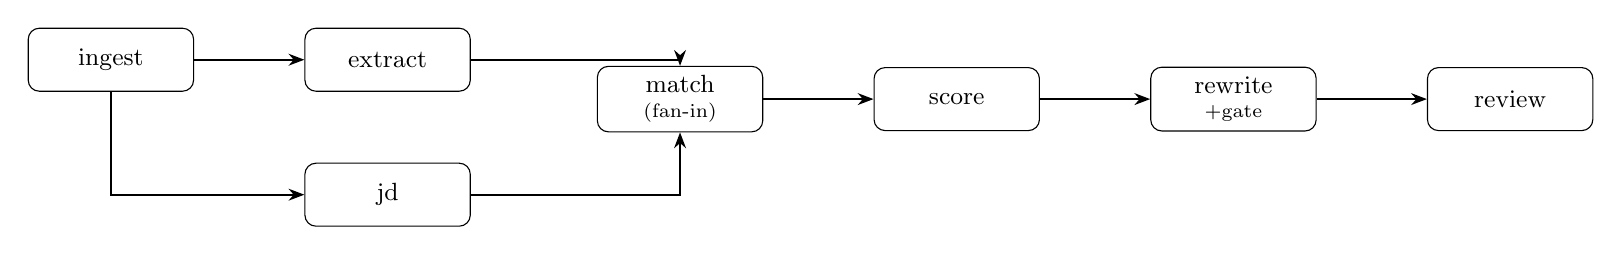
\begin{tikzpicture}[
  node distance=0.9cm and 1.4cm,
  box/.style={draw, rounded corners, minimum width=2.1cm, minimum height=0.8cm, align=center, font=\small},
  arr/.style={-{Stealth[length=2mm]}, thick}
]
\node[box] (ingest) {ingest};
\node[box, right=of ingest] (extract) {extract};
\node[box, below=of extract] (jd) {jd};
\node[box, right=1.6cm of extract, yshift=-0.5cm] (match) {match\\[-2pt]\scriptsize(fan-in)};
\node[box, right=of match] (score) {score};
\node[box, right=of score] (rewrite) {rewrite\\[-2pt]\scriptsize+gate};
\node[box, right=of rewrite] (review) {review};

\draw[arr] (ingest) -- (extract);
\draw[arr] (ingest.south) |- (jd.west);
\draw[arr] (extract) -| (match);
\draw[arr] (jd) -| (match);
\draw[arr] (match) -- (score);
\draw[arr] (score) -- (rewrite);
\draw[arr] (rewrite) -- (review);
\end{tikzpicture}
\caption{The seven-node pipeline. \texttt{extract} and \texttt{jd} run in parallel off a shared
\texttt{ingest} step; \texttt{match} is a defer-until-both-inputs-ready barrier, not a
first-input-wins race, so it never sees a partially-populated state. The reviewer node
independently re-checks the provenance invariant on the shipped rewrite rather than trusting the
gate's own accounting.}
\label{fig:pipeline}
\end{figure}

The system is a seven-node graph (Figure~\ref{fig:pipeline}) built on a directed-graph
orchestration library \citep{langgraph2024}: \texttt{ingest} $\to$ \texttt{extract} and
\texttt{ingest} $\to$ \texttt{jd} run in parallel, both feeding a \texttt{match} node that acts as a
genuine fan-in barrier (it is deferred until \emph{both} predecessor paths have completed, not
triggered by whichever arrives first -- a distinction that matters operationally, since the
job-description branch is typically far shorter than résumé extraction and a naive
any-of-predecessors trigger would race \texttt{match} against a résumé that has not finished
parsing). \texttt{match} feeds \texttt{score} (C2), which feeds \texttt{rewrite} (C3's gate is
applied here, internally, before the node returns), which feeds \texttt{review} -- a node whose
only job is to independently re-run the provenance-invariant check against the résumé the pipeline
is about to return, and report the result (\texttt{invariant\_ok}, plus the specific values that
failed, if any) rather than silently trusting that the gate upstream did its job correctly.

\textbf{The provenance chain (C1).} At ingestion, every extracted span of source text is assigned
a stable identifier (\texttt{prov\_id}) recording its document, character offsets, and raw text.
Every value-bearing field the extraction stage produces carries a sibling \texttt{*\_prov} field
listing the \texttt{prov\_id}s that support it. This is not metadata added after the fact: it is
attached during extraction, propagated through matching (a matched job requirement's ``present''
status carries the \texttt{prov\_id} of the résumé span that satisfies it), and is what the
rewrite gate checks against. The invariant this chain exists to enforce: \emph{at the output of the
rewrite stage, every hard-content token -- skill, tool, organization name, number, date -- must
trace to at least one \texttt{prov\_id} whose source text supports it}. This is checked twice: once
inside the rewrite node (rejecting and reverting individual failing edits before the node returns),
and again, independently, by the reviewer node against the final shipped résumé.

\textbf{Calibrated scoring (C2).} The matcher produces a five-dimensional raw feature vector
(keyword coverage, semantic similarity, fuzzy coverage, must-have coverage, nice-to-have coverage)
against the job description's parsed requirements. Rather than reporting a function of this vector
directly as a $0$--$100$ score, a calibrator is fit against the actual output of a self-hostable,
rule-based ATS simulator \citep{atsscreener} run over the same résumé--job-description pairs, using
the simulator's job-description-dependent scoring dimension as the regression target (see
Section~\ref{sec:results} for why the composite dimension is the wrong target). The calibrator is
a simple linear model (Ridge regression); the point of C2 is not the model family, it is that the
score is anchored to what an actual ATS does, not to an unvalidated proxy.

\textbf{The rewrite gate (C3).} The rewriter is prompted with the source résumé as the explicit
sole source of truth, instructed to reorder, rephrase, select, and emphasize existing content but
never invent skills, tools, employers, titles, metrics, dates, or certifications, and asked to
leave a requirement honestly unsatisfied rather than fabricate coverage for it. This prompt is
deliberately \emph{not} the safety mechanism. Every value in the rewriter's raw output is checked,
deterministically and without any further LLM call, against the source résumé's provenance chain:
values already present in the source (reordered, rephrased) are accepted; genuinely new
hard-content values that do not resolve to a supporting \texttt{prov\_id} are rejected, and the
rewritten résumé is repaired to remove them before it ships. The number of rejections, over the
number of total proposed edits, is reported as the \texttt{fabrication\_rate} -- a metric that
exists specifically so that ``the gate is doing something'' is falsifiable rather than assumed.

\section{Experimental Setup}

\textbf{Backends.} The primary inference backend for every result in this paper is
\texttt{gemini-3.1-flash-lite} \citep{gemini}, a hosted commercial API, used under its free-tier
quota. Every result is additionally validated against a locally-hosted open model served via
Ollama \citep{ollama}: \texttt{qwen2.5:14b} \citep{qwen25} for the fabrication-gate and pipeline
results, and \texttt{gemma3:4b} for the calibration result specifically (Section~\ref{sec:results},
C2) -- the two open models used are not identical across tasks, and we report each task's actual
open-model backend rather than a single unified name. All backends use genuine
schema-constrained decoding: Ollama's \texttt{format} parameter for the local models, and Gemini's
\texttt{responseSchema} for the hosted backend.

\textbf{Datasets.} Extraction quality (C1) is evaluated over 300 gold-labeled résumés drawn from
three sources: 120 synthetic résumés with exact-by-construction field labels and provenance spans
(an upper bound on achievable performance, since templated text is cleaner than real résumés); 30
hand-labeled résumés drawn from a real-world résumé corpus, labeled by the paper's authors and
\emph{not} independently verified; and 150 résumés from a public, independently human-annotated
named-entity-labeled résumé dataset (the trustworthy real-data number, since its annotations are
independent of this system and its authors). Calibration (C2) uses 199 usable résumé--job-description
pairs (out of 200 requested; one dropped for missing engine output), drawn by pairing résumés and
job descriptions from public résumé and job-posting corpora, weighted 80\% toward same-category
pairings so there is genuine keyword overlap to find. The fabrication benchmark (C3) uses 30
corpus-backed pairs built the same way, with the pressure on the rewriter (which job-description
requirements are absent from the résumé) generated by the system's own job-description-analysis
and matching stages rather than a hand-written adversarial list.

\section{Results}
\label{sec:results}

\subsection{C1 -- Extraction Quality}

Table~\ref{tab:c1} reports field-level F1 across the three gold sets on the primary backend. No
comparable open-model extraction run exists for this table: the open-model backends in this paper
were evaluated on job-description analysis, matching, and rewriting (Sections
\ref{ssec:c2}--\ref{ssec:c3}), not on extraction against a labeled gold set, so C1 is reported for
the primary backend only and we do not imply a cross-model comparison that was not measured.

\begin{table}[h]
\centering
\caption{Extraction quality (C1), \texttt{gemini-3.1-flash-lite}. Long-text fields (résumé
summaries) are reported separately from named-entity fields, since prose is rewritten by the
extractor rather than copied verbatim and would otherwise mask entity-level performance.}
\label{tab:c1}
\begin{tabular}{lccccc}
\toprule
Gold set & $n$ scored / total & skills F1 & job title F1 & institution F1 & prov.\ accuracy \\
\midrule
1a: synthetic (upper bound) & 120 / 120 & 0.999 & 1.000 & 1.000 & 0.894 \\
1b: real corpus (unverified) & 25 / 30 & 0.443 & 0.931 & 0.693 & -- \\
1c: public, human-annotated & 143 / 150 & 0.753 & 0.935 & 0.917 & 0.874 \\
\bottomrule
\end{tabular}
\end{table}

The headline number is Table 1c (public, human-annotated, independent of this system's authors):
skills F1 $0.753$ (precision $0.802$ / recall $0.749$), job title F1 $0.935$, institution F1
$0.917$, certification F1 $0.802$, and a provenance-attachment accuracy of $0.874$ -- meaning 87.4\%
of extracted field values could be traced to the correct supporting span in the source document.
The gap between the synthetic upper bound (skills F1 $0.999$) and the real, human-annotated set
(skills F1 $0.753$) is real-world résumé messiness (inconsistent formatting, abbreviations,
implicit skills), not a defect specific to this pipeline; the synthetic result establishes that the
pipeline is correct when the input is unambiguous.

\textbf{Extraction reliability limitation.} $7/150$ (1c) and $5/30$ (1b) documents -- $12/300$
overall, 4\% -- failed extraction outright rather than scoring poorly, and are excluded from the
table above rather than counted as zero. Every failure traced to the same root cause, confirmed by
direct reproduction against the API and by two independent full evaluation runs producing
\emph{identical} failures on the \emph{identical} document identifiers (temperature is 0 for
extraction, so this is deterministic, not sampling noise): the model enters a degenerate
repetition loop when a résumé's employment dates are formatted ambiguously across multiple lines
(e.g.\ \texttt{"03/2015\textbackslash nto\textbackslash n07/2017"}), repeating a malformed
ISO-timestamp fragment until it exhausts its output-token budget, at which point the response is
truncated mid-string and is not valid JSON. We consider this a genuine, reportable finding about
the primary backend's reliability on this task, not an artifact to average away: the system's
per-document failure isolation (each document's extraction is independently try/excepted) meant
this degraded to ``12 documents skipped and logged,'' not a crashed evaluation run, but it is a real
gap between measured throughput and successful throughput that a deployment would need to plan for.

\subsection{C2 -- ATS-Calibrated Scoring}
\label{ssec:c2}

\begin{table}[h]
\centering
\caption{Calibration quality (C2), held-out split (139 train / 60 held-out of 199 usable pairs),
target is the ATS simulator's job-description-dependent scoring dimension.}
\label{tab:c2}
\begin{tabular}{lcccc}
\toprule
Backend (job-desc.\ analysis) & $n$ usable & Calibrated MAE / $\rho$ & Cosine MAE / $\rho$ & Wall-clock \\
\midrule
\textbf{Gemini (\texttt{gemini-3.1-flash-lite})} & \textbf{199/199} & \textbf{3.25 / 0.333} & \textbf{27.58 / 0.229} & \textbf{836s (14min)} \\
Open model (\texttt{gemma3:4b}, Ollama) & 199/200 & 3.17 / 0.328 & 26.00 / 0.168 & 39{,}162s (10.9h) \\
\bottomrule
\end{tabular}
\end{table}

The calibration target is deliberately the ATS simulator's job-description-\emph{dependent} scoring
dimension, not its five-dimension composite score: on this corpus the composite is dominated by
résumé-intrinsic quality signals (formatting, section completeness) that do not vary with the job
description, and calibrating against it produces a target against which our own match features
correlate \emph{negatively}. Restricting the target to the dimension that actually depends on the
job description flips every correlation positive and is the number we report as headline.

Calibrated MAE and Spearman $\rho$ are within run-to-run noise of each other across backends (a
repeated run of the open-model pipeline alone produced $\rho \in \{0.328, 0.440\}$ on different
held-out splits of the same 199 pairs), so the roughly 3-point spread in Table~\ref{tab:c2} is not
a meaningful backend effect. The finding worth reporting is throughput: the hosted backend
completes the same 199-pair calibration run \textbf{47$\times$ faster} in wall-clock time, because
it is not bottlenecked on CPU-bound local token generation. Both backends beat the raw-cosine
baseline by a wide margin in rank correlation ($\rho$ 0.33 / 0.23 calibrated vs.\ 0.23 / 0.17
cosine), which is the scale-free comparison that matters given the cosine baseline emits a
0--100 score while the true target range is narrow (mean 13.4, s.d.\ 4.9).

\subsection{C3 -- Fabrication Gate}
\label{ssec:c3}

\begin{table}[h]
\centering
\caption{Fabrication gate (C3), 30 corpus-backed adversarial pairs. ``Gate OFF'' is the rewriter's
raw output under prompt grounding alone; ``Gate ON'' is the same output after the provenance-verified
gate. Gate-ON is 0 by construction on both backends -- the claim under test is whether that holds
independent of which model drives the rewriter.}
\label{tab:c3}
\begin{tabular}{lcccc}
\toprule
Backend (rewriter) & Pairs scored & Gate OFF & Gate ON & Mean fabrication rate \\
\midrule
\textbf{Gemini (\texttt{gemini-3.1-flash-lite})} & \textbf{30/30} & \textbf{40} & \textbf{0} & \textbf{0.248} \\
Open model (\texttt{qwen2.5:14b}, Ollama) & 30/30 & 31 & 0 & 0.407 \\
\bottomrule
\end{tabular}
\end{table}

Gate-ON is 0 on both backends: across every one of the 30 adversarial pairs, on two different
rewriter models, no unsourced hard-content value reached the shipped output. This is the central
claim of C3, and Table~\ref{tab:c3} demonstrates it is a property of the deterministic gate, not a
behavior that happens to hold for one particular model's generation style. The two backends differ
in how much fabrication the gate had to catch: the hosted backend proposed more unsourced additions
in absolute count (40 vs.\ 31) despite a lower mean fabrication rate concentrated over fewer
affected pairs (10/30 vs.\ 14/30) -- a rewriter that fabricates more aggressively on the subset of
pairs where it fabricates at all, not a more conservative one overall. Rejected examples are
substantive, not near-miss paraphrases: invented skills (\emph{Microsoft Word}, \emph{Microsoft
Excel}, \emph{Project Management}), invented soft-skill claims (\emph{Team Leadership},
\emph{Marketing Event Coordination}), and invented bullet-level claims (\emph{``Performed tasks
requiring basic math and numerical proficiency using 10-key''}) on the hosted backend; invented
employers, fabricated metrics, and a leaked prompt-reasoning artifact on the open-model backend.
None of these reached the shipped output on either backend.

\textbf{Ablation.} Replacing the provenance-resolved gate with the cheaper substitute a
provenance-free system would have to use -- a plain case-insensitive substring search for the
proposed value anywhere in the source document's raw text -- catches 36 of the 40 rejections the
real gate makes, but \textbf{misses 4}: additions that appear, in some form, somewhere in the
source text but are not actually supported by it in the place the rewriter used them. This is the
measured value of resolving to an actual span rather than checking bag-of-words presence.

\subsection{Pipeline-Level Result}

Running the full seven-node pipeline end-to-end on a single résumé and job description, the hosted
backend completes in 15.7s versus 268.5s for the open-model backend (17$\times$) -- consistent with
the throughput difference observed in C2. On this specific run, the reviewer node's independent
provenance check caught a case the individual-edit gate check alone would not have surfaced as
cleanly: the extraction stage produced a plain year (\texttt{"2020"}) reformatted into a full,
non-matching ISO timestamp (\texttt{"2020-01-01T00:00:00Z"}), which fell just under the
fuzzy-match threshold used to resolve provenance and was correctly flagged
(\texttt{invariant\_ok=False}) rather than shipped silently -- and, on the same run, the gate
independently rejected a genuinely fabricated skill (\emph{``Data Engineering''}) the rewriter
proposed with no supporting source span. Both outcomes are the reviewer and gate doing their job
correctly on a real, unstaged generation; the open-model run on the same input showed neither
condition, since its extraction did not exhibit the date-reformatting behavior described above.

\section{Limitations}

\textbf{The primary backend has a deterministic extraction failure mode.} As detailed in
Section~\ref{sec:results} (C1), 4\% of extraction calls on the primary hosted backend
failed via a reproducible degenerate-generation loop on a specific class of ambiguous date
formatting. This is contained by the system's per-document error isolation but is a real
throughput cost a production deployment on this backend would need to account for, and it is not
a failure mode we observed on the open-model backend.

\textbf{The hosted backend's zero API cost is a free-tier artifact, not a design property.} Every
result in this paper using \texttt{gemini-3.1-flash-lite} incurred \$0 in billed API spend, but
only because the evaluation volume stayed inside the provider's free-tier daily quota. This is
qualitatively different from the open-model results, which are self-hosted compute and are
genuinely free at any scale. Reproducing the hosted-backend results at larger scale would require
either a paid tier or distributing calls across additional free-tier accounts.

\textbf{No fine-tuned small-model comparison.} A fine-tuned small extraction model is a
plausible alternative to prompting a general-purpose LLM at scale; this system does not include
one, and the extraction backbone's vLLM/constrained-decoding path exists in the codebase but was
never exercised on a CUDA-equipped host during this evaluation.

\textbf{Semantic-similarity thresholds are untuned.} The matcher's cosine-similarity bands used to
classify a requirement as present, weakly present, or absent are the design's original proposed
defaults; no sweep against a labeled match-quality set has been performed, and they should be
treated as provisional.

\textbf{Fabrication benchmark scale.} The C3 result is measured over 30 adversarial pairs. The
gate-ON$=0$ result held exactly across all 30 pairs on two backends, which is meaningful evidence
of a structural guarantee rather than a sample-dependent behavior, but a larger benchmark would
strengthen the claim further, particularly around the mean fabrication-rate estimate, which is
sample-size-sensitive in a way the gate-ON count is not.

\section{Conclusion}

We presented a résumé-optimization system built around a provenance identifier space that survives
unbroken from document ingestion through a rewrite stage, a match score calibrated against a real
ATS simulator's output rather than an embedding-similarity proxy, and a deterministic rewrite gate
that rejects any proposed value the provenance chain cannot support. Evaluated primarily on a
hosted \texttt{gemini-3.1-flash-lite} backend, the system achieves 0.874 provenance-attachment
accuracy and 0.753 skills F1 on an independently human-annotated gold set, a calibrated match score
with $\rho=0.333$ against a real ATS engine's output, and -- the central claim -- zero unsourced
additions reaching a shipped rewrite across every adversarial pair tested, a guarantee we confirmed
is backend-independent by reproducing it on a locally-hosted \texttt{qwen2.5:14b}. We also reported,
rather than elided, a genuine and reproducible extraction-reliability limitation of the primary
backend, because a system whose safety property is ``fabrication cannot ship'' should hold itself
to the same standard when reporting its own failure modes.

\bibliography{refs}

\end{document}
